Wolfenstein 3D, released on May 5th, 1992, established the First Person Shooter genre. The game design, powered by an engine enabling beautiful 256 color graphics, speed, high framerate, clever I.A, crisp sound effects, and engaging music, was universally acclaimed. Within a year more than 100,000 units had been sold over the mail\footnote{The game was distributed via shareware.}, bringing fame and a little bit of fortune to the team who built it, id Software.\\
\par
\begin{figure}[H]
\centering
\fullimage{action_packed.png}
\end{figure}
\par
But the many fans did not stop at beating the game. Driven by a desire to modify it and make their own characters and maps, they started to explore and reverse engineer. Within a few months the asset formats were well known and people released mods\footnote{MODified version.} with altered graphics, sounds effects, music, and maps. However, the core of the game, the 3D engine and the secrets of its speed, remained mostly unknown.\\
\\
It was kept secret for an obvious reason: a powerful engine is an essential asset for a gaming company. As a means to outperforming competitors, it's good business practice to keep other programmers clueless. This allows for maintaining a technological advantage, making betters games and generating more profit.\\
\\
However, a few people within id Software did not see things that way. Instead of going along with what was common sense, they wanted to embrace players' enthusiasm and fully open the source code to the public. After much internal debate, id Software did the unthinkable: on July 21st, 1995 they uploaded a zip archive on \emph{ftp.idsoftware.com} containing the full source code of the engine with instructions to build it\footnote{They were not totally crazy, they had built a game engine making Wolfenstein 3D obsolete: Doom was released on December 10, 1993}.\\

 \begin{fancyquotes}
   Programming is not a zero-sum game. Teaching something to a fellow programmer doesn't take it away from you. I'm happy to share what I can, because I'm in it for the love of programming.\\
   \\
\textbf{John Carmack - Programmer}
 \end{fancyquotes}\\
\\
Opening the code did much more than enable programmers. It had two unforeseen consequences.\\
\\
First, it allowed the software to live long after the target hardware and operating system dissapeared. With access to the source, programmers were able to maintain and port the engine to new hardware and operating systems. Twenty years after the release of Wolfenstein 3D, you can still play the game on anything with a CPU, some RAM, and a framebuffer. \\
\\
Second, it created a window back in time to 1991. Having reviewed complex engines such as Quake III and Doom III on \emph{fabiensanglard.net}, I thought I would have merely skimmed over the Wolfenstein 3D engine and its "simple" raycasting technology. When I took a deeper look out of curiosity, something struck me and I could not stop. The more I read, the more I came to realize how the target machine, the IBM PC, was designed for office work, not for gaming. It was meant to crunch integers and display static images for word processing and spreadsheet applications. This is the story this book is trying to tell, what id Software\footnote{A few other companies, such as Origins and LucasArts where also doing amazing things. I focus on id because we have the source code!} did in 1991 was not just program a machine. What they did was re-purpose a tool built to do office work and turn it into the best gaming platform in the world.\\
\\
But why go through so much trouble? After all, if you were a game company and you wanted to make video games, you had video game consoles dedicated to this very specific task. The Genesis, the Super NES, and the Neo-Geo had sprite engines which despite limitations such as size and number allowed movement of something on the screen by simply updating its $(x,y)$ coordinates. They were able to easily generate smooth animation at 60 frames per second, had controllers, had an audio system for sound and music, and were homogeneous (e.g: all SNES were the same). If you still really wanted to use a personal computer for a game, why not use an Amiga 500 which was packed with coprocessors designed for animation?\\
\\
The reason fits in one word: Framebuffer. The kind of game id Software wanted to create could not be done with a sprite engine or tricks from a Copper\footnote{Nickname of a powerful Amiga co-processor allowing operations at hsync level.}. They wanted to shake the gaming world by providing an immersive experience in three dimensions. In order to do that they needed to draw a full screen, pixel by pixel, in a framebuffer before it was sent to the monitor. \\
\par
To draw all these pixels they needed a powerful CPU and a PC outperform any console on the market. No Amiga\footnote{Jimmy Maher advances an interesting theory in his book "The Future was here: The Commodore Amiga": People wanted to play First Person Shooter, which the Amiga architecture did not allow. This inability ultimately provoked the downfall of Commodore's best seller.}, even with their co-processor, could rival a PC in terms of raw power.
\par
\begin{figure}[H]
\centering
  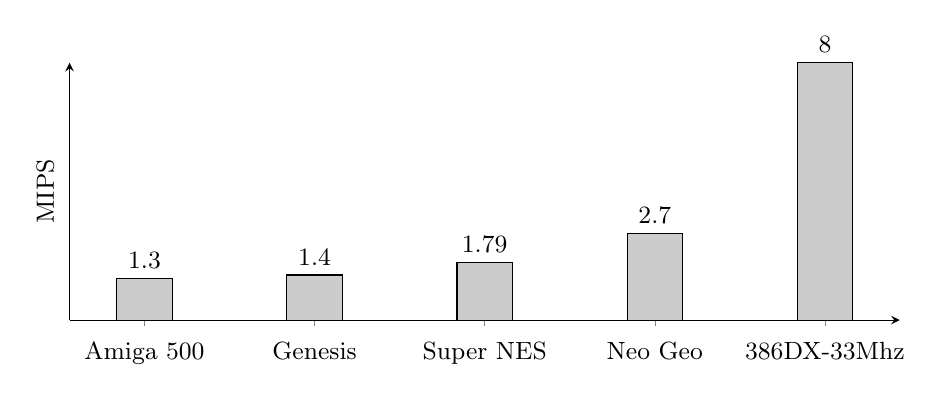
\begin{tikzpicture}[font=\small]
    \begin{axis}[
      width=\textwidth,
      height=0.4\textwidth,
      ybar=6pt,
      bar width=20pt,
      ylabel={MIPS},
      ymin=0,
      ytick=\empty,
      xtick=data,
      axis x line=bottom,
      axis y line=left,
      enlarge x limits=0.11,
      symbolic x coords={Amiga 500, Genesis, Super NES, Neo Geo,386DX-33Mhz},
      xticklabel style={anchor=base,yshift=-\baselineskip},
      nodes near coords={\pgfmathprintnumber\pgfplotspointmeta}
    ]
      \addplot[fill=black!20,draw=black] coordinates {
        (Amiga 500,1.3)
        (Genesis,1.4)
        (Neo Geo,2.7)
        (Super NES,1.79)
        (386DX-33Mhz,8)
      };
    \end{axis}
   \end{tikzpicture}
   \caption{Consoles Vs PC, CPU comparison with MIPS\protect\footnotemark \protect\footnotemark.}
   \label{fig:ems_xms_layout}
 \end{figure}
 % Latex footnote I HATE YOU !!!!!!
 \addtocounter{footnote}{-1}
 \footnotetext{Million Instructions Per Second.}
 \stepcounter{footnote}
 \footnotetext{The Amiga 500, Genesis, and Neo-Geo have a Motorola 68000 CPU respectively running at 7.16 MHz, 7.6 MHz, and 12 Mhz. The Super NES uses a WDC 65816 CPU which is a 8/16 bit version of a 6502 running at 3.58 MHz.}


 
With its fast CPU and 256K framebuffer, a 1991 PC looked promising at first. Except according to the user manual there were three seemingly impossible\footnote{The title of this book could have easily be "The Impossible Machine".} obstacles to overcome:\\
\begin{itemize}
\item The video system (called VGA) could not double buffer. It was not possible to have smooth animations without ugly artifacts called "tears" on the screen.
\item The CPU could only do integer operations but the mathematics required for 3D calculations involved keeping track of fractions.
\item The PC Speaker, the default sound device, could only produce square waves. A bunch of "beeps" which were more annoying than anything else.
\end{itemize}
On top of these major blockers lied fuve major difficulties:\\
\begin{itemize}
\item The RAM addressing mode was not flat but segmented, resulting in complex and error prone pointer arithmetics.
\item VGA pixels were not square: the framebuffer was stretched vertically when
transferred to the screen.
\item The audio ecosystem was fragmented: various sound systems had different capabilities and expectations.
\item The machine could only address 1MB of RAM. To go beyond you had to enter a fragmented eco-system of drivers.
\item The bus was slow and I/O with the VRAM was a bottleneck. It was impossible to write a full framebuffer each frame.
\end{itemize}

Overall, it looked like the machine was \emph{doom}ed to do boring things. But many around the world did not accept that and tinkered with the hardware to achieve unexpected results. How they did it is the raison d'\^etre of this book. I've chosen to divide this book in three chapters. By first showing the hardware constraints, I hope programmers will develop an appreciation for the software and how it navigates obstacles, sometimes turning limitations into advantages.
\begin{itemize}
\item Chapter I: The Hardware. The five components of a PC from 1991.
\item Chapter II: The Team\footnote{This is an engineering book: The description is logistic. For the human aspect read David Kushner's chef d'oeuvre: "Masters of Doom''}. The people pushing the edges.
\item Chapter III: The Software. Wolfenstein 3D game engine.
\end{itemize}
\par
\bu{Trivia :} The name "Wolfenstein 3D" was inspired by the 1981 Apple II title "Castle Wolfenstein" from Silas Warner. The Apple version was stealth oriented (Wolfenstein "Profound Carnage" style was a clear departure from the original theme) but really stood out thanks to its unprecedented use of digitized voices. Initially the team believed that they would be unable to use the Wolfenstein name due to trademark issues, and came up with multiple possible titles, only to discover that the original developer, Muse Software, had gone out of business several years earlier and let the trademark lapse, leaving them free to name their game Wolfenstein 3D.

\begin{figure}[H]
\centering
\scaledimage{0.9}{intro_wolf_appleii.png}
%\caption{Castle Wolfenstein (Apple II version)}
\end{figure}


\begin{figure}[H]
\centering
\scaledimage{0.9}{CastleWolfensteinAppleII.png}
\end{figure}
